\section{Statistical unit and exploratory paired uncertainty}
\label{sec:paired-uncertainty}

An external benchmark collection contains many forecast origins but not an
equal number of independent replications. Several origins of one series share
most fitting observations, and the forecast leads belong to one jointly
generated future block. Treating every lead or origin as an independent
replication would make the reported precision depend on how densely the same
series was evaluated. We therefore first average the available origins within
a series and then give each admitted series equal weight. This choice defines
the population summary being described; it is not merely a computational
convenience for obtaining a narrower interval.

Let $L_{so}(A)$ be a loss for method $A$ at origin $o$ of series $s$, and let
$\mathcal O_s$ contain that series' admitted origins. Define
\begin{equation}
 \bar L_s(A)=|\mathcal O_s|^{-1}\sum_{o\in\mathcal O_s}L_{so}(A),
 \qquad d_s(A,B)=\bar L_s(A)-\bar L_s(B).
 \label{eq:paired-series-loss}
\end{equation}
The collection mean difference is
\begin{equation}
 \bar d(A,B)=N^{-1}\sum_{s=1}^N d_s(A,B).
 \label{eq:paired-collection}
\end{equation}
For MASE and MSIS, a negative value favors $A$. A signed coverage difference
has no universal direction of improvement: increasing coverage by making
intervals wider can worsen their usefulness. Coverage differences are retained
in the complete evidence, but are not labeled loss reductions.

\subsection{Collection admission and the denominator of a comparison}
\label{sec:collection-admission}

Table~\ref{tab:collection-inventory} identifies the source inventory and the
actually admitted comparison. The weekly exclusions are recorded under the
combined reason of nonfinite observations or no eligible origin; that category
does not support attributing every exclusion to a particular history-length
threshold. The monthly exclusions are exact duplicates. All excluded identities
remain visible in the numerical index, so the denominator is not reconstructed
from successful forecasts alone. A comparison conditioned on eligibility does
not describe source series for which the specified fitting protocol could not
produce an origin.

\begin{table}[htbp]\centering\small
\caption{Source inventories and admitted external evaluation units. Each origin has twelve methods; the weekly and monthly horizons differ. Point values count one scalar per method and lead, not all three quantiles.}
\label{tab:collection-inventory}
\begin{tabular}{lrrrrrr}\toprule
Collection & $H$ & Source & Admitted & Excluded & Origins & Point values\\\midrule
M4 Weekly & 13 & 359 & 294 & 65 & 882 & 137,592\\
M3 Monthly & 18 & 1428 & 1422 & 6 & 3547 & 766,152\\
Total & -- & 1787 & 1716 & 71 & 4429 & 903,744\\\bottomrule
\end{tabular}\end{table}


The external comparison contains 4,429 origins and twelve methods, yielding
\externalpathcount{} method-origin forecast paths: 10,584 weekly paths with thirteen leads and
42,564 monthly paths with eighteen leads, or \externalpointcount{} individual point predictions. The same future targets
are scored for every method at an origin. Counting those repeated method-target
pairs as independent experimental outcomes would confuse computational volume
with inferential sample size. The series-level mean in
Equation~\ref{eq:paired-collection} uses 294 weekly or 1,422 monthly observations,
not the number of scalar predictions. The separate fifteen selected development
cases are retained for comparison with the original proposal; they are not
added to either external collection's inference denominator.

\subsection{What was resampled, and what was not}
\label{sec:paired-resampling}

One bootstrap draw samples $N$ complete series identities with replacement and
averages their paired differences. The two methods are never sampled
independently. All origins already belonging to a sampled series remain
together through its within-series mean. M4 Weekly and M3 Monthly are analyzed
separately, because pooling their differently selected series and scale
denominators would change the estimand. With resampled identities
$S_1^*,\ldots,S_N^*$, the bootstrap statistic is
\begin{equation}
 \bar d^*=N^{-1}\sum_{i=1}^N d_{S_i^*},\qquad
 C_{.95}=[Q_{.025}(\bar d^*),Q_{.975}(\bar d^*)].
 \label{eq:paired-bootstrap}
\end{equation}
The computation uses 10,000 local PCG64 draws, linear empirical quantiles and
seed 20261105 plus a stable collection-specific offset. Identical resampled
indices are used across comparisons within a collection. Batch size bounds
memory consumption without changing the random sequence.

This uncertainty analysis was specified after the original outcomes were
available. It does not refit a forecaster, alter an expert weight, change a
validation schedule, remove an unfavorable series or obtain new external
data. Its intervals are unadjusted and exploratory. Under independent
representative series and regularity conditions, a series bootstrap can
describe sampling variation in a mean difference. The intervals here are not
finite-sample distribution-free coverage guarantees. Related industries,
shared source processes or other dependence between nominally distinct series
can invalidate independent-series resampling. Exact whole-sequence
deduplication removes a clear duplication defect, but does not prove that all
remaining series are statistically independent.

\subsection{Comparisons and their different interpretations}
\label{sec:paired-outcomes}

Table~\ref{tab:paired-main} reports ValidationMix minus two informative controls.
RecencyMean isolates whether a temporally validated combination improves beyond
the matching recency-only memory rule. AutoTheta is a separately implemented
statistical forecast and supplies a stronger external alternative on several
metrics. The controls answer different questions; improvement over the
recency ablation cannot be presented as superiority over the complete roster.
The complete numerical file additionally retains ContextMemoryCV and AutoETS,
all signed coverage comparisons, means, medians and loss-direction counts.

\begin{table}[htbp]\centering\small
\caption{ValidationMix minus each control after averaging available origins within each series. Unadjusted exploratory 95\% paired-series intervals describe the admitted collection, not population-wide superiority.}
\label{tab:paired-main}
\begin{tabular}{lllrrr}\toprule
Collection & Control & Loss & Difference & 95\% interval & Lower loss\\\midrule
Weekly & RecencyMean & MASE & $-0.025337$ & $[-0.033914,-0.017227]$ & 190/294\\
Monthly & RecencyMean & MASE & $-0.009154$ & $[-0.013176,-0.005173]$ & 589/1422\\
Weekly & AutoTheta & MASE & $-0.022065$ & $[-0.037521,-0.008272]$ & 155/294\\
Monthly & AutoTheta & MASE & $0.052154$ & $[0.032437,0.073112]$ & 689/1422\\
Weekly & RecencyMean & MSIS & $-0.383808$ & $[-0.431160,-0.334374]$ & 252/294\\
Monthly & RecencyMean & MSIS & $-0.063788$ & $[-0.088692,-0.040255]$ & 589/1422\\
Weekly & AutoTheta & MSIS & $0.835230$ & $[0.650853,1.038115]$ & 49/294\\
Monthly & AutoTheta & MSIS & $2.521379$ & $[2.364504,2.673453]$ & 267/1422\\
\bottomrule\end{tabular}\end{table}


The MASE differences favor ValidationMix over RecencyMean in both collections,
and their paired intervals exclude zero under the stated resampling procedure.
This is evidence about these measured aggregate differences. It does not
identify which component of the selector caused the difference, prove
out-of-collection generalization or establish that most individual series
improve. On M3 Monthly, only 589 of 1,422 series have strictly lower MASE than
RecencyMean, even though the collection mean is lower. Unequal magnitudes of
improvements and regressions, together with equal outcomes, can produce that
combination. Mean difference and win fraction are different summaries.

Against AutoTheta, the point-error direction depends on the collection.
ValidationMix has the favorable weekly mean difference, while AutoTheta has
the favorable monthly difference. AutoTheta also has lower MSIS in both
collections. Thus the experiment does not identify a universally preferable
forecast distribution. It identifies a bounded improvement of a temporally
validated combination relative to its recency control, while retaining a
stronger alternative for monthly point error and both interval scores.

\begin{figure}[htbp]\centering
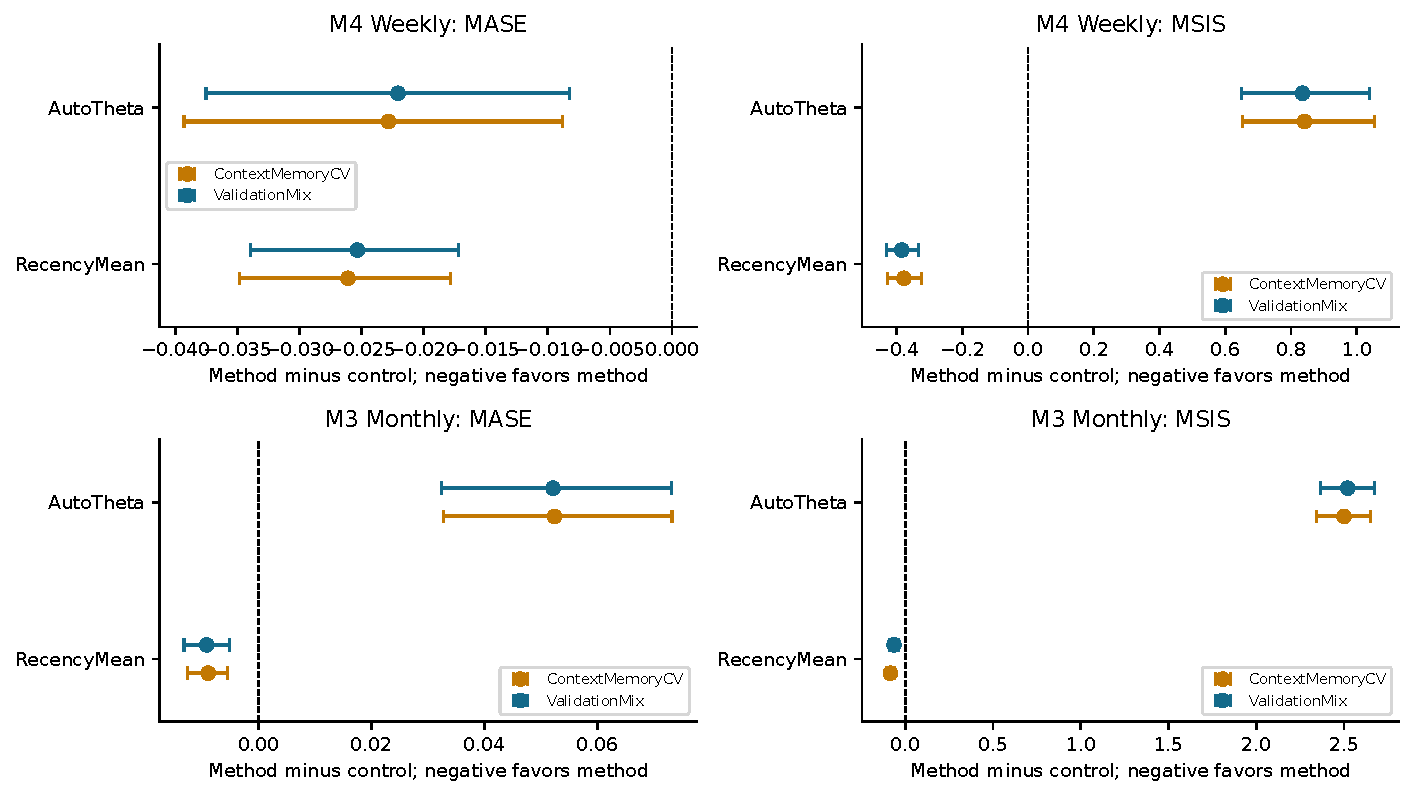
\includegraphics[width=\textwidth]{paired-series-intervals.pdf}
\caption{Exploratory paired-series intervals for the two temporally validated
combinations. Negative loss differences favor the combination; separate panels
retain differences between collections, controls and point versus interval losses.}
\label{fig:paired-intervals}\end{figure}

Figure~\ref{fig:paired-intervals} places both combinations against matching
controls, rather than displaying only a favorable subset. The MSIS panels
show that a point-error improvement does not guarantee a better distributional
forecast. Figure~\ref{fig:paired-directions} complements the mean differences
with complete series-level direction counts. Equal-loss series remain in the
denominator. Removing them would change the displayed fraction and could
create an impression of broad individual gains that the complete collection
does not support.

\begin{figure}[htbp]\centering
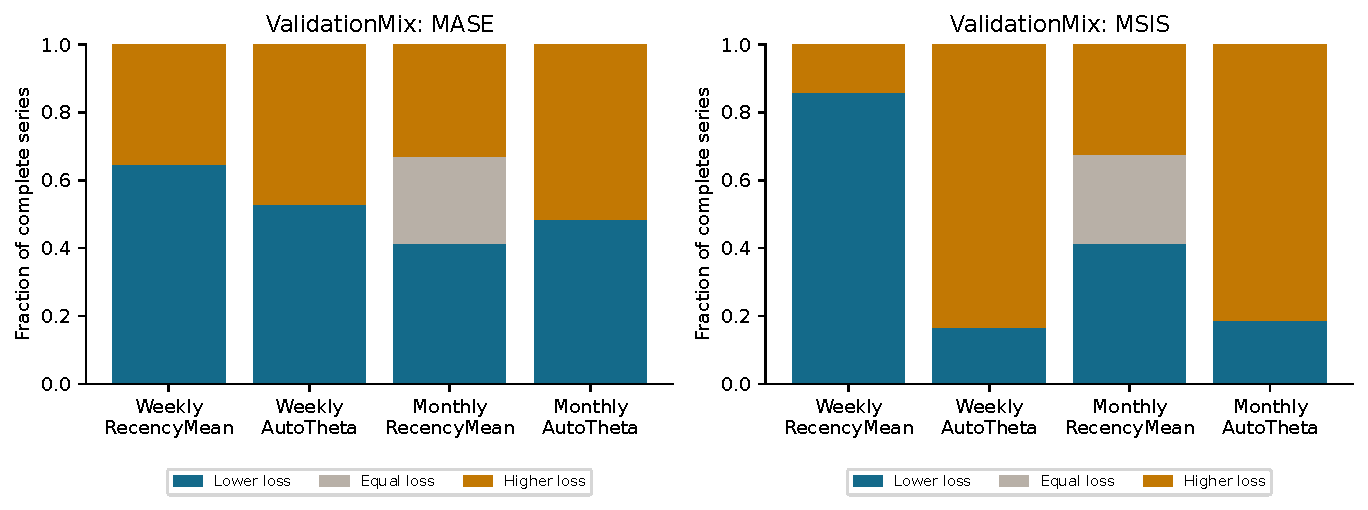
\includegraphics[width=\textwidth]{paired-series-directions.pdf}
\caption{Fractions of admitted series with lower, equal or higher ValidationMix
loss after averaging origins. Aggregate mean gains need not imply that most
series improve, especially when loss magnitudes are unequal.}
\label{fig:paired-directions}\end{figure}

\subsection{Causality, selection and attribution}
\label{sec:paired-causality}

The outer forecast at query origin $q$ may select a rule using a historical
validation origin $o$ only when its entire target block is already observed:
\begin{equation}
 o+H\leq q.
 \label{eq:completed-validation}
\end{equation}
Every historical expert fit uses observations available at its own origin.
The query's reserved targets enter neither an expert fit nor the selection
criterion. Figure~\ref{fig:causal-order} depicts this information order; its
positions illustrate the constraint and are not a measured timing result.
Using a recently started but incomplete target block would leak future
information into the selector even if its features were computed from a valid
prefix. The completion condition therefore applies to outcomes as well as
features.

\begin{figure}[htbp]\centering
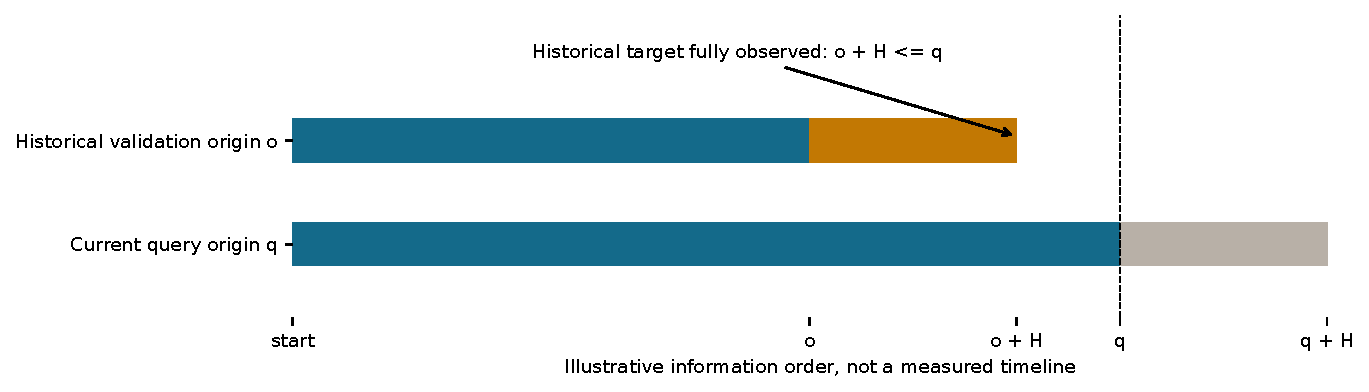
\includegraphics[width=\textwidth]{causal-validation-order.pdf}
\caption{Illustrative information order for historical validation and a current
query. A historical target must be completely observed before it can inform
selection; the gray current target remains reserved for evaluation.}
\label{fig:causal-order}\end{figure}


\begin{algorithm}[htbp]
\caption{Temporally completed candidate selection. Every expert forecast and
validation target used to choose a combination is available before the current
reserved target block begins.}
\label{alg:temporal-selection}
\begin{algorithmic}[1]
\Require Observed prefix $y_{1:n}$, horizon $H$, fixed candidates $\mathcal C$
\State Construct the fixed historical origin schedule and cache expert paths
\For{each historical query origin $q$}
\State Retain earlier origins $o$ satisfying $o+H\leq q$
\State Use the query only when at least three completed origins are available
\For{each candidate $c\in\mathcal C$}
\State Fit its weights from the completed historical memories only
\State Score its combined path on the query block using the query's prefix scale
\EndFor
\EndFor
\State Select minimum mean validation loss; break ties by the fixed grid order
\State With no eligible query, use the explicitly defined recency-only fallback
\State Fit the selected rule's current weights from all completed prefix memories
\State Return the weighted current expert path without observing $y_{n+1:n+H}$
\end{algorithmic}
\end{algorithm}

Algorithm~\ref{alg:temporal-selection} separates the selection protocol from
its candidate weight formula. A grid containing contextual softmax weights and
regularized stacking does not let either candidate train on its own validation
outcomes. The fallback is part of the declared algorithm, not an exclusion of
short or inconvenient prefixes after their errors are observed. The final
outer block remains reserved regardless of which candidate is selected.

Causal data access prevents one important validity defect, but does not remove
selection uncertainty. A fixed finite candidate grid can still overfit a small
set of completed historical blocks. ContextMemoryCV and ValidationMix can
choose different candidates at different outer origins, and an aggregate
gain is the outcome of the complete procedure. It is not an isolated estimate
of the context kernel's causal contribution. The recency-only and equal-weight
rules provide informative ablations; neither equals a fully crossed experiment
in which every stacking, regularization and context choice is independently
randomized or disabled while the selection budget is otherwise identical.

The resampling analysis consequently leaves the original scope intact. It
adds uncertainty and distributional summaries to frozen forecasts, rather
than converting a retrospective comparison into a preregistered trial.
Independent code recomputes the reported differences from full-precision
audit paths and confirms that two analysis processes produce identical JSON
bytes. This supports computational reproducibility. The externally admitted
series, fixed temporal protocol and explicit unfavorable controls bound the
scientific interpretation of the resulting means and intervals.
